\documentclass[sigconf]{acmart}
% Cleaning
\pagestyle{fancy} % removes running headers
\settopmatter{printacmref=false} % Removes citation information below abstract
\renewcommand\footnotetextcopyrightpermission[1]{} % removes footnote with conference information in first column
\pagestyle{plain} % removes running headers
\fancyhead{}
\settopmatter{printacmref=false, printfolios=false}
% Copyright
\setcopyright{none}
% \setcopyright{acmcopyright}
% \setcopyright{acmlicensed}
% \setcopyright{rightsretained}
% \setcopyright{usgov}
% \setcopyright{usgovmixed}
% \setcopyright{cagov}
% \setcopyright{cagovmixed}
\settopmatter{printacmref=false} % Removes citation information below abstract
\acmDOI{}


\setlength{\parskip}{0pt}
\setlength{\parsep}{0pt}
\setlength{\headsep}{0pt}
\setlength{\topskip}{0pt}
\setlength{\topmargin}{0pt}
\setlength{\topsep}{0pt}
\setlength{\partopsep}{0pt}
%\linespread{0.95}
\usepackage{mdwlist}
\usepackage{amsmath}
\usepackage{graphicx}
\usepackage{booktabs} % \toprule etc.; harmless if acmart already loads it
\usepackage{array}    %  needed for >{\raggedright\arraybackslash} in the tables
\usepackage{pgfplots}
\pgfplotsset{compat=1.17}
% [Claude] chart colours: a colour-blind-safe blue/orange pair (validated for CVD separation and contrast)
\definecolor{chartblue}{HTML}{2A78D6}
\definecolor{chartorange}{HTML}{EB6834}


% [Claude] the draft macros \prov and \note are removed: \note clashed with a command acmart already defines
% ("Command \note already defined"), and neither is used any more.
\begin{document}
% [Claude] \mbox keeps the title on one line; without it the footnote mark pushes "Data" onto a second line.
\title{\mbox{Evaluating Ocean Drift Prediction from Wind and Location Data}}
\titlenote{Code and data: \url{https://github.com/jakecush1/autonomous-pilot-ML}}
\author{Jake Cushway}
\affiliation{
  \institution{University of Victoria}
  \city{Victoria}
  \country{Canada}
}
\email{jakecush1@uvic.ca }

\author{Rowan Hall}
\affiliation{
  \institution{University of Victoria}
  \city{Victoria}
  \country{Canada}
}
\email{rowanhall@uvic.ca }


\begin{abstract}
DataXplorer, an uncrewed surface vehicle (USV) serving as a weather station off Half Moon Bay, California, must stay within 10~nautical miles (NM) of the retired NOAA buoy 46012. We forecast its position one hour ahead from onboard wind and GPS data alone, comparing an LSTM and a Transformer with persistence and linear regression on 94~days of 1-minute telemetry. On unseen deployments the LSTM is best, with a median error of 213~m, 30\% below persistence. Code and data: \url{https://github.com/jakecush1/autonomous-pilot-ML}.
\end{abstract}

\keywords{Uncrewed surface vehicle, drift prediction, LSTM, transformer}
\maketitle
\pagestyle{empty}

\section{Introduction}
Pilots keep DataXplorer on station by watching its position and repositioning it; a reliable drift forecast would let them intervene only when needed. Operational drift models such as GNOME~\cite{zelenke2012gnome} and leeway models~\cite{breivik2011leeway} move an object with a fitted fraction of the wind on top of forecast currents. We instead learn the drift from the USV's own record, and test whether an LSTM~\cite{hochreiter1997lstm} and a Transformer~\cite{vaswani2017attention} improve on persistence and linear regression.


\section{Research Questions}
\noindent\textbf{RQ1.} Do the sequence models predict the USV's position one hour ahead more accurately than the baselines, and which model is best? Answering this shows whether learning patterns within the past hour, such as the drift turning, is worth the extra complexity. In response, we benchmark the LSTM and Transformer against persistence and linear regression by their error on the final test set.


\noindent\textbf{RQ2.} How much does wind contribute to predicting drift? We expected wind to be the main driver of drift, since it both pushes on the USV and drives the surface current.
Leeway models treat it as such~\cite{breivik2011leeway}, and it is one of only two inputs our models use. In response, we measure how often the USV drifts with the wind, how much of the drift a linear fit on the wind explains, and how the linear regression's error changes without its wind features.




% [Claude] RQ3 switched from the hyperparameter study (not run) to error by wind strength, at Jake's request (Nov 18 2026).
\noindent\textbf{RQ3.} Does each model's error depend on wind strength? A pilot needs to know whether a model's advantage holds in all conditions. In response, we split the final-test error of every model by the mean wind over its input hour.

\begin{table}[t]
\centering\footnotesize
\caption{Dataset statistics over all nine deployments.}
\label{tab:dataset}
\begin{tabular}{@{}ll@{}}
\toprule
Deployments            & 9 (Apr 17 -- Nov 16, 2026) \\
Records (1 per minute) & 135{,}234 (93.9 days) \\
% With GPS fix           & 121{,}406 (84.3 days) \\
Missing values         & 11.0\% of records \\
Motor off              & 50.3\% of minutes \\
% Motor-on episodes      & 592 \\
Valid drift minutes    & 66{,}803 (46.4 days) \\
Samples (dev.\ / final test) & 30{,}303 / 3{,}920 \\
% Input features         & 4 per minute $\times$ 60 minutes \\
% Target (next 60 min)   & movement east, north (m) \\
% \quad median / 90th pct / max & 763 / 1{,}469 / 2{,}575 \\
Drift speed (median)   & 0.44\,kn \\
Wind speed (mean / max)& 10.0 / 28.2\,kn \\
Wind direction         & 54\% from the NW \\
\bottomrule
\end{tabular}
\end{table}


\section{Dataset}
The data was collected directly from DataXplorer by Open Ocean Robotics at the site of NOAA buoy 46012; we exported only the channels this experiment needs (time, GPS position, wind speed and direction, and motor power), and the files are in our repository. They cover nine deployments from April to November 2026 (Table~\ref{tab:dataset}). A minute is valid when the motor is off, the vessel moves slower than 3~kn (faster means a tow) and no value is missing after gaps of up to 5~minutes are interpolated. A sample needs 120 consecutive valid minutes: the past hour is the input, with four features per minute (movement and wind push, each east and north), and the movement over the next hour, read from later GPS positions, is the target. This gives 34{,}223 samples. No public benchmark covers this vessel, so its own record at the site of use is the most relevant data; it lacks winter and measured currents.

% ===========================================================================
% The headings follow the manual (4.4 Baselines, 4.5 Evaluation Strategy and Metrics, 4.6 Results).
% Marks: baselines 5%, strategy and metrics 5%, results with attribution and discussion 50%, reproducibility 20%.
% ===========================================================================


\section{Baselines}

% NOTE (manual 4.4): for each baseline say how it works, why it is a fair competitor, its hyperparameters,
% the library, and a reference. Milestone 3 has the full descriptions, so a sentence or two each is enough.
We compare the LSTM and Transformer with two baselines. All four models use the same samples, cleaning and metric.

\textbf{Persistence} predicts that the next hour's movement repeats the last hour's. It needs no training and has no hyperparameters. It is the bar every model must beat.

\textbf{Linear regression} predicts the next hour's movement from six numbers summarising the past hour: the movement, the current wind and the mean wind, each east and north. Like a leeway model~\cite{breivik2011leeway}, it moves the USV linearly with the wind, on top of a term for its past drift, so it tests whether a linear model suffices before turning to nonlinear ones. We use \texttt{LinearRegression} from scikit-learn, which has no hyperparameters to tune.


% [Claude] filled in at Jake's request (Nov 18 2026); facts from src/models/nn_models.py
% (LSTM: 2 layers, 64 hidden, dropout 0.2, last hidden state -> output; Transformer: 2 encoder layers, d=64,
% 4 heads, dropout 0.1, sin/cos positions, mean-pool -> output).
\textbf{LSTM and Transformer} are the models under test. Both read the past hour minute by minute: the LSTM~\cite{hochreiter1997lstm} carries a memory along the sequence, while the Transformer~\cite{vaswani2017attention} lets every minute attend to every other. Each has two layers of width 64 and is implemented in PyTorch.


% [Claude] Table 2 replaced by a bar chart (final test set, evaluation/results/results.json "test").
% The old table (Oct 16-23 numbers) is in git history.
\begin{figure}[t]
\centering
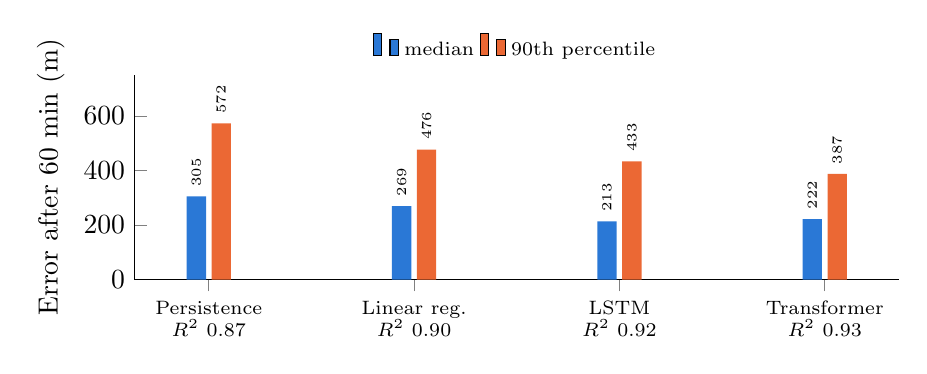
\begin{tikzpicture}
\begin{axis}[
    ybar, bar width=7pt,
    scale only axis, width=0.8\columnwidth, height=2.6cm,  % axis box only; the y label adds ~1 cm
    ymin=0, ymax=750, ytick={0,200,400,600},
    ylabel={Error after 60 min (m)},
    xtick={1,2,3,4},
    xticklabels={{Persistence\\$R^2$ 0.87}, {Linear reg.\\$R^2$ 0.90}, {LSTM\\$R^2$ 0.92}, {Transformer\\$R^2$ 0.93}},
    xticklabel style={align=center, font=\scriptsize},
    enlarge x limits=0.12,
    axis lines*=left,
    nodes near coords,
    nodes near coords style={font=\tiny, rotate=90, anchor=west},
    legend style={at={(0.5,1.02)}, anchor=south, legend columns=2, font=\scriptsize, draw=none},
]
\addplot[fill=chartblue, draw=none] coordinates {(1,305) (2,269) (3,213) (4,222)};
\addplot[fill=chartorange, draw=none] coordinates {(1,572) (2,476) (3,433) (4,387)};
\legend{median, 90th percentile}
\end{axis}
\end{tikzpicture}
\Description{Vertical bar chart of the median and 90th-percentile endpoint error on the final test set:
persistence 305 and 572 m (R-squared 0.87), linear regression
269 and 476 m (0.90), LSTM 213 and 433 m (0.92), Transformer 222 and 387 m (0.93).}
\caption{Error after 60 minutes on the final test set.}
\label{fig:results}
\end{figure}


\section{Evaluation Strategy and Metrics}

\textbf{Splits.} Neighbouring samples overlap almost completely, so instead of a random split we split by deployment in time order: April--October form the development set (30{,}303 samples) and November the final test set (3{,}920 samples), scored once after all settings were fixed. In place of $n$-fold cross-validation, the latest development deployment (Oct 16--23) is held out for validation, so that training always precedes validation and test in time.

\textbf{Metric.} The endpoint error is the distance in metres between the predicted and the true position after 60 minutes. We report its median (a typical miss), its 90th percentile (a bad case) and $R^2$, the share of the variation in the movement that a model explains. As the output is a position, classification metrics such as accuracy or F1 do not apply.

% [Claude] filled in at Jake's request (Nov 18 2026); settings from src/models/nn_models.py (lr 1e-3, batch 256,
% up to 80 epochs, patience 10, seed 0). No hyperparameter search was run.
\textbf{Hyperparameters.} The LSTM and Transformer are trained with Adam~\cite{kingma2015adam} (learning rate $10^{-3}$, batches of 256) on the squared error, stopping once the validation error has not improved for 10~epochs. These settings are untuned defaults; tuning them is future work.

\section{Results and Discussion}



% NOTE (manual 4.6): one part for each RQ: state the answer, give the numbers, then say why.
% No result that does not answer an RQ. This section is 50% of the mark, so it gets the most space.

% [Claude] Nov 18 2026: RQ1 now on the FINAL TEST SET (data/holdout, Nov 2-16), scored once; train Apr-Oct 13,
% early stopping on Oct 16-23, seed 0. Numbers: evaluation/results/results.json ("test"). The old red Oct 16-23
% numbers are in git history. Still one seed per model, so the 9 m LSTM-Transformer gap may be noise.

% [Claude] RQ1 answer with the final-test numbers, in the example paper's pattern.
\textbf{RQ1: do the sequence models beat the baselines?} Figure~\ref{fig:results} shows that both sequence models outperform both baselines on the final test set. The LSTM has the lowest median error, 213~m, 30\% below persistence and 21\% below linear regression, while the Transformer has the lowest 90th percentile, 387~m, 32\% below persistence; both reach an $R^2$ of 0.92--0.93. This can be attributed to the sequence models reading the past hour minute by minute, so they see the drift turn or slow, whereas persistence assumes the last hour repeats and linear regression sees only its totals. Persistence still more than halves the error of assuming no drift (747~m), because the current changes slowly (RQ2), and linear regression beats it only through its wind features. With one seed per model, the 9~m gap between the two may be noise.



% [Claude] RQ2 answer, in the manual's 4.6 pattern (answer, numbers, then why). Numbers from
% src/linear_fits/drift_vs_wind.py 60 (development set, 25,640 motor-off minutes, drift over 60 min).
% Earlier placeholder, kept in case there is room for the run without wind:
% NOTE: show the error with and without wind for each learned model, as a small table or a bar chart.
% \textbf{RQ2: how much does wind contribute?} We retrain each learned model with the two wind features removed. \prov{Without wind, the median error of the [model] changes from [A]~m to [B]~m.} \prov{[Why.]}
\textbf{RQ2: how much does wind contribute?} Figure~\ref{fig:withwind} shows that wind steers the drift but does not dominate it. On the development set, the USV drifts within $\pm45^\circ$ of downwind 47\% of the time, against 25\% if wind had no effect; below 5~kn the share is 20\%, no better than chance, and above 15~kn it reaches 87\%. This can be attributed to the balance between wind and current: in light wind the current sets the direction, and only a strong wind overcomes it. The drift along the wind grows at 4.2\% of the wind speed, near the 1--4\% windage GNOME assumes~\cite{zelenke2012gnome}, and is turned about $20^\circ$ right of downwind, as the Coriolis effect predicts. Still, wind speed explains little of the drift speed ($R^2 = 0.11$), and the wind vector about a quarter of the drift ($R^2 = 0.23$). For prediction, removing the wind features from the linear regression raises its median error on the final test set from 269 to 301~m (90th percentile 476 to 587~m), but by only 2~m on the validation week (see RQ3).

\begin{figure}[t]
\centering
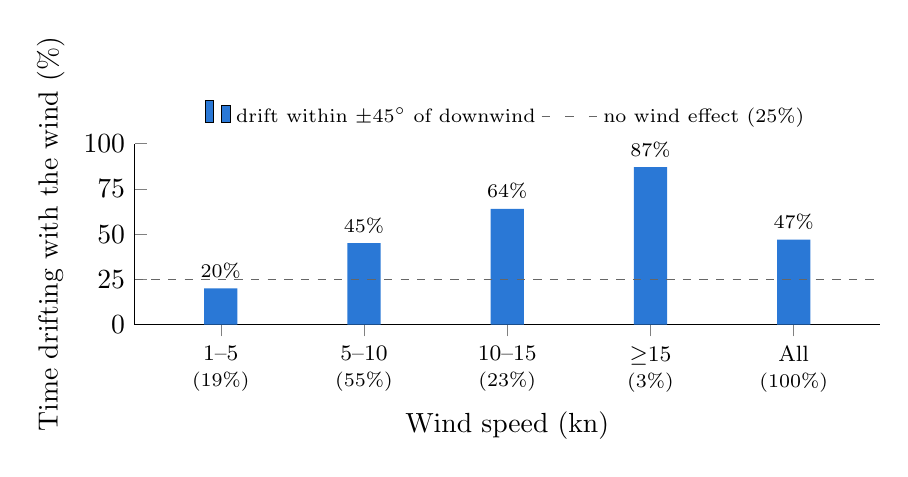
\begin{tikzpicture}
\begin{axis}[
    ybar, bar width=12pt,
    scale only axis, width=0.78\columnwidth, height=2.3cm,  % axis box only; the y label and ticks add ~1.3 cm
    ymin=0, ymax=100, ytick={0,25,50,75,100},
    ylabel={Time drifting with the wind (\%)},
    xlabel={Wind speed (kn)},
    xtick={1,2,3,4,5},
    xticklabels={{1--5\\\scriptsize(19\%)}, {5--10\\\scriptsize(55\%)},
                 {10--15\\\scriptsize(23\%)}, {$\geq$15\\\scriptsize(3\%)}, {All\\\scriptsize(100\%)}},
    xticklabel style={align=center, font=\footnotesize},
    enlarge x limits=0.15,
    axis lines*=left,
    nodes near coords={\pgfmathprintnumber{\pgfplotspointmeta}\%},
    nodes near coords style={font=\scriptsize},
    legend style={at={(0.5,1.03)}, anchor=south, legend columns=2, font=\scriptsize, draw=none},
]
\addplot[fill=chartblue, draw=none] coordinates {(1,20) (2,45) (3,64) (4,87) (5,47)};
\addlegendentry{drift within $\pm45^\circ$ of downwind}
\addlegendimage{line legend, dashed, black!60}
\addlegendentry{no wind effect (25\%)}
\draw[dashed, black!60] (rel axis cs:0,0.25) -- (rel axis cs:1,0.25);
\end{axis}
\end{tikzpicture}
\Description{Bar chart of the share of time the USV drifts within 45 degrees of downwind:
20\% at 1--5 kn, 45\% at 5--10 kn, 64\% at 10--15 kn, 87\% above 15 kn and 47\% overall,
against 25\% expected if wind had no effect on direction.}
\caption{Time the USV drifts within $\pm45^\circ$ of downwind, by wind speed (share of minutes in brackets).}
\label{fig:withwind}
\end{figure}

% [Claude] RQ3 answer (src/evaluate/error_by_wind.py, evaluation/results/error_by_wind.json; final test set).
\textbf{RQ3: does the error depend on wind strength?} Table~\ref{tab:wind} splits the final-test error by wind strength. Both sequence models beat persistence in every band, by 18--40\% in median error, so their advantage holds across conditions. It is largest in light wind (LSTM 211~m against 350~m), which can be attributed to the current: when it sets the drift and turns with the tide, persistence carries the old direction forward, while the sequence models see the turn. In strong wind, however, the Transformer keeps its 90th percentile at 378~m while the LSTM's rises to 546~m; with one seed per model and no wind above 15~kn in the validation week, this needs confirming. Contrary to RQ2's suggestion, linear regression's wind features lower its median error below 15~kn (by about 50~m) but not above.

\begin{table}[!ht]
\centering\footnotesize
\caption{Final-test error by wind: median / 90th pct.\ (m).}
\label{tab:wind}
\begin{tabular}{@{}lccc@{}}
\toprule
Model (samples) & $<$10~kn (1{,}064) & 10--15~kn (1{,}740) & $\geq$15~kn (1{,}116) \\
\midrule
Persistence & 350 / 637 & 283 / 484 & 313 / 628 \\
Linear regression & 286 / 458 & 244 / 418 & 289 / 531 \\
Linear reg., no wind & 333 / 546 & 297 / 578 & 286 / 614 \\
LSTM & \textbf{211} / 404 & \textbf{208} / \textbf{393} & 226 / 546 \\
Transformer & 217 / \textbf{376} & 232 / 396 & \textbf{211} / \textbf{378} \\
\bottomrule
\end{tabular}
\end{table}

% NOTE: 20% of the mark. Give the one command that reproduces every table and figure, the fixed seeds,
% the run time, and where the results are written.
\textbf{Reproducibility.} The command \texttt{bash quickstart.sh} installs the pinned dependencies and reruns every step, from the raw telemetry in \texttt{data/} to every number, table and figure reported here (written to \texttt{evaluation/results/}). Seeds are fixed, so a rerun gives identical numbers; the full run takes about 5~minutes on a laptop.

% NOTE: if there is room, close with one sentence: what a pilot can rely on, and what comes next.

\bibliographystyle{ACM-Reference-Format}
\bibliography{bibliography.bib}

\end{document}
